\documentclass[12 pt]{exam}
\usepackage{graphicx, enumitem, amsmath, amssymb}
\graphicspath{ {./images/} }
\usepackage{tikz, pgfplots}
\usetikzlibrary{shapes,arrows}
%\usepackage{Minion Pro}
\printanswers

\title{1.6 Solving the Consumer's Problem - Practice Problems (Answers)}
\author{Ryan Safner}
\date{ECON 306 - Fall 2019}

\begin{document}

\maketitle

You can get utility from consuming Soda $(s)$ and Hot dogs $(h)$, according to the utility function:

\begin{equation*}
u(s,h)=\sqrt{sh}\end{equation*}

The marginal utilities are:

\begin{align*}
MU_s&=0.5s^{-0.5}h^{0.5}	\\
MU_h&=0.5s^{0.5}h^{-0.5} \\ \end{align*}

You have an income of \$12, the price of Soda is \$2, and the price of a Hot dog is \$3. Put Soda on the horizontal axis and Hot dogs on the vertical axis.

\begin{questions}
  \question What is your utility-maximizing bundle of Soda and Hot dogs?
  \begin{solution}
  	Use the definition of the optimum: 
\begin{align*}
MRS_{s,h}&=\frac{p_s}{p_h} & & \text{Definition of the optimum}\\
\frac{MU_s}{MU_h}&=\frac{p_s}{p_h} && \text{Definition of MRS on left}\\
\frac{0.5s^{-0.5}h^{0.5}}{0.5s^{0.5}h^{-0.5}}&=\frac{(2)}{(3)} & & \text{Plugging in what we know}\\
		\frac{0.5}{0.5}s^{(-0.5-0.5)}h^{(0.5-[-0.5])} &=\frac{2}{3} && \text{Using exponent rules for division}\\
		s^{-1}h^{1} &=\frac{2}{3} && \text{Simplifying and cancelling}\\
		\frac{h}{s}&=\frac{2}{3} && \text{Using exponent rules for negative exponents}\\
	h&=\frac{2}{3}s && \text{Multiplying both sides by} s\\	
\end{align*}

So we know that we will be buying $\frac{2}{3}$ sodas for every 1 hot dog. This is the optimal ratio of consumption between the two goods. 

To find the exact quantities of $s$ and $h$, use the budget constraint:

\begin{align*}
p_ss +p_hh &=m & & \text{The budget constraint equation}\\
2s + 3h &=12 & & \text{Plugging in what we are given}\\
2s + 3(\frac{2}{3}s)&=12 & & \text{Plugging in what we found relating }b \text{ to } a\\
2s+2s&=12 & & \text{Multiplying}\\
4s&=12 & & \text{Adding}\\
s&=3 & & \text{Dividing by } 4\\	
\end{align*}

Now that we know the quantity of sodas, we can use our knowledge of the ratio of sodas to hot dogs to find the quantity of hot dogs. 
\begin{align*}
h&=\frac{2}{3}s\\
h&=\frac{2}{3}(3)\\
h&=2\\ 	
\end{align*}

	\end{solution}


  \question How much utility does this provide?
  
  \begin{solution}
  How much utility do we get? Plug our optimal bundle into the utility function: 
\begin{align*}
u(s,h)&=\sqrt{sh}\\
u(s,h)&=\sqrt{(3)(2)}\\
u(s,h)&=\sqrt{6}\\	
\end{align*}

  \end{solution}
\end{questions}

If we wanted to graph the indifference curve, we need to solve for $h$ (the good on the vertical axis). 
	
	\begin{align*}
	u(s,h)&=\sqrt{sh}\\
	\sqrt{6}&=\sqrt{sh}\\
	6&=sh\\
	\frac{6}{s}&=h\\	
	\end{align*}

Same with the budget constraint to graph: 
\begin{align*}
p_ss + p_hh &= m\\
2s+3h&=12\\
3h&=12-2s\\
h&=4-\frac{2}{3}s\\
\end{align*}

\begin{center} 
	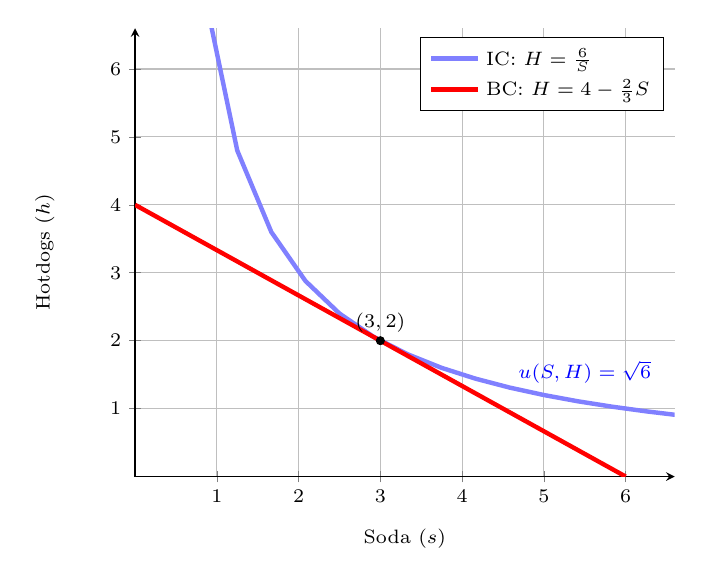
\begin{tikzpicture}\scriptsize 
	\begin{axis}[
		axis lines=middle, 
		enlarge x limits={rel=0.1, upper},
		enlarge y limits={rel=0.1, upper},
		every axis y label/.style={at={(axis description cs:-0.2,0.5)},rotate=90,anchor=north},
		every axis x label/.style={at={(axis description cs:0.5,-0.1)},anchor=north},
	%legend pos=outer north east,
	legend cell align=left, 
	xlabel=Soda ($s$),
	ylabel=Hotdogs ($h$),
	xtick={1, 2,...,6},
	ytick={0,1,...,6},
	grid=major,
	ymin=0,
	xmin=0,
	ymax=6,
	xmax=6
]
	\addplot[ultra thick, color=blue!50, domain=0:10, samples=25]{6/x};
	\addlegendentry{IC: $H=\frac{6}{S}$};
	\draw[blue] (axis cs:5.5,1.25)node[above]{$u(S,H)=\sqrt{6}$};
	\addplot[ultra thick, red, domain=0:6, samples=25]{4-.666666*x};
	\addlegendentry{BC: $H=4-\frac{2}{3}S$};
	\draw[fill=black] (axis cs:3,2)circle(0.05cm)node[above]{$(3,2)$};
\end{axis}
\end{tikzpicture}
\end{center} 

\end{document}